\chapter{Soll-Konzept und Implementierung}

\section {Analyse der bereits erweiterten Suchen}

Als Referenzmodelle für die Umsetzung des Kundenwunsches dienen die erweiterten Suchen der Rezepte, der Materialstückliste und der Dokumente, da die gewünschten Felder hier bereits implementiert wurden. Folglich können für die Anpassung der Suchoberfläche der Spezifikationen Informationen zum Vorgehen und der Umsetzung aus diesen Referenzmodellen gewonnen werden.

Zunächst wird der Aufbau des General Views untersucht, da hier viele Parallelen zu der Spezifikation erkennbar sind.
Bei der Betrachtung fällt auf, dass die Verwaltungsdaten im Layout der Referenzmodelle deckungsgleich aufgebaut sind. Alle \ac{ui}-Elemente dieses Abschnitts werden von einem Transportcontainer umfasst. Ein Transportcontainer definiert ähnlich wie ein View einen Bereich, in dem die untergeordnete Entitäten nach im Container definierten Regeln angeordnet werden.

Zu den untergeordneten Elementen gehört das Suchkriterium changed on, für das ebenfalls ein Transportcontainer angelegt wurde. In diesem Transportcontainer befinden sich zwei Eingabefelder, damit für das Änderungsdatum auch ein Zeitraum eingetragen werden kann. Vor den Eingabefeldern wurde für das Suchkriterium auch ein Label angelegt, welches die Eingabefelder im \ac{ui} beschriftet. Darauf folgen das Label und das Eingabefeld für das Suchkriterium changed by.

Den Labels wird mithilfe von \acs{otr} Texten ein Titel zugewiesen. Das Online Text Repository ist ein zentraler Ablagebereich für Texte im SAP-System. Vorteil der \acs{otr} Texte ist unter anderem, dass sich ihre Bezeichnung an die verwendete Sprache der Suchoberfläche anpasst.  

Neben den \acs{otr}-Texten ist bei der Analyse der \ac{ui}-Elementattribute aufgefallen, dass den gleichen  \ac{ui}-Bausteinen bei unterschiedlichen Referenzmodellen dieselben prozentualen Breiten und Ausrichtungen wie zum Beispiel linksbündig zugeteilt wurden. Aufgrund dieser Kongruenz empfiehlt es sich, den Aufbau und die Konfiguration der \ac{ui}-Elemente der Referenzmodelle für die Suchoberfläche der Spezifikation zu übernehmen. 

Bei der Untersuchung der Verbindungen zwischen den Web-Dynpro-Entitäten bemerkt man, dass die \ac{ui}-Strukturen der Referenzmodelle für die neuen Felder um vier weitere Komponenten erweitert wurden. Auffällig ist die Besonderheit, dass zwei der Komponenten in allen Referenzmodellen mit der Bezeichnung LOW und HIGH beginnen. Nachforschungen haben gezeigt, dass die dafür verantwortliche Methode auch bei der Spezifikation verwendet wird. Folglich sollten für die \ac{ui}-Struktur der Spezifikation zwei Komponenten mit beginnend LOW und HIGH angelegt werden, da andernfalls die Methode die Eingabefelder nicht erkennen und verarbeiten kann.

%Beim Vergleichen der Verbindungen zwischen Layout, Content und Componentcontroller, fällt auf dass die UI-Strukturen um weitere Felder, die auf der Suchoberfläche zusehen sind, erweitert wurden. Auffällig ist die Besonderheit, dass bei der normalen View für die Eingabe des Zeitraums aufgrund der zwei Inputfelder auch zwei Komponenten bei der Struktur benötigt werden, die mit LOW und HIGH beginnnen. Nachforschungen haben gezeigt, dass das an der Methode ... liegt. In der Methode, welche auch bei der Spezifikation verwendet wird, werden die zwei Datumsangaben zu einem Zeitraum verknüpft. Dafür müssen die Komponenten der UI Strukutr mit den Bezeichnungen LOW und HIGH beginnen, da andernfalls die Felder von der Methode nicht erkannt und somit auch nciht verknüpft werden können.

%Beim der Untersuchung  der \ac{ui}-Strukturen der Referenzmodelle bemerkt man, dass die \ac{ui}-Strukturen der Refenzmodelle für die neuen Felder um weitere Komponenten erweitert wurden. Die Komponenten haben zwar unterschiedliche Typen aufgrund von unterschiedlichen Datenquellen, aber immer die gleiche Beschreibung: Last Changed By und Last Changed On. Folglich müssen für die neuen Komponeten die Typen mit der gleichen Beschreibung gefunden und der \ac{ui}-Struktur der Spezifikation zugewiesen werden.\change{mit Kommentaren S. 23 abgleichen, nicht ganz rund}

Bei der Analyse des Range Views der Referenzmodelle ist die BUILD\_UP Methode aufgefallen. Diese wurde für die Einbindung der neuen Suchkriterien in die Suchoberfläche um 2 weitere Programmabschnitte erweitert. Dort werden die neuangelegten Komponenten zur Definition der Eingabedaten wiederverwendet. Für die Programmierung der erweiterten Suche der Spezifikation stellt der Code eine ausgezeichnete Vorlage dar, die es bei der Anwendung für das Objekt der Spezifikation anzupassen und zu erweitern gilt. 

Die Interfaces und Windows der Web-Dynpro-Component blieben bei den Referenzmodellen für die Funktionalität unverändert und sollten daher auch bei der Web-Dynpro-Component der Spezifikation unverändert bleiben.

%Anpassen
Bei der Untersuchung des Suchmodells der Materialstückliste in dem \ac{es}-Cockpit stellt man fest, dass die verwendeten Datenbanktabellen und Modellanfrageattribute im Vergleich zur Spezifikation andere Bezeichnungen haben, aber das Vorgehen bei der Modifikation des Suchmodells auf die Spezifikationsänderungen übertragen werden kann.

Zunächst muss für die Anbindung der Datenbanktabellen die Datenquelle in den Modellknoten festgehalten werden. Anschließend müssen die für die Suchanfrage benötigten Suchkriterien zu den Modellanfrageattributen hinzugefügt werden. Die Untersuchung der Suchmodelle für die \ac{plm}-Objekte Dokumente und Rezepte bestätigten diese Erkenntnisse.









\section{Umsetzung des Kundenwunsches}


Für die Verwirklichung des Kundenwunsches hat die Analyse der Referenzmodelle gezeigt, dass neben der Erweiterung der Suchoberfläche im Frontend auch die Modifikation der Suchmodelle im Backend notwendig ist. 
%Bei der Umsetzung wird auf die von den Referenzmodellen gewonnnenen Erkenntnisse zurückgegriffen.

%In der Dreisystemlandschaft\change{In SAPTEC als SAP-Softwarelogistik bezeichnet} bestehend aus Entwicklungs-,Qualitätssischerungs und Produktivsysteme, werden die Änderungen zunächst nur in den Entwicklungssystemen implementiert, damit der Produktivbetrieb der Systeme beim Kunden unverändert bleibt.

Zunächst werden die erforderlichen Anpassungen im Backend dargestellt. Hier wurden mit den Enterprise-Search-Tools die zur Spezifikation gehörenden Suchmodelle und Konnektoren angepasst.

Damit die Daten der neuen Suchkriterien aus der Datenbanktabelle ausgelesen werden können, wurde der Modellknoten SPEC\_KEY, um die Anfrageattribute UPDNAMS und UPDDATS erweitert. Im Modellknoten eines Suchmodells lassen sich die Spalten der Datenbanktabelle, die angebunden werden sollen, auswählen. Daraufhin wurden die zuvor genannten Attribute auch in der Modellanfrage des Suchmodells selektiert, um für die später hinzugefügten Suchfelder im \ac{plmwui} eine Suche im Index oder der Datenbank zu ermöglichen. 

Nach dem Anpassen des Suchmodells wurde über das \ac{es}-Cockpit der zum Suchmodell dazugehörige Konnektor aktualisiert. Der Konnektor stellt eine Instanz des Modells dar und verbindet den Suchdatenprovider der Applikation mit der Enterprise Search. Ohne den Konnektor ist die Suche nach Spezifikationen nicht möglich. 

%Nachdem das Backend erfolgreich geändert wurde, kann das Front-End für die Normale - und die Range View mithilfe des \ac{abap} Editors angepasst werden. Hierzu wurde zunächst die \ac{ui}-Struktur, um die Komponente UPDNAMS von Typ ESEUPDNAM und die Komponenten LOW\_UPDDATS, HIGH\_UPDDATS und UPDDATS vom Typ ESEUPDDAT erweitert. Dabei wurden die Typen der beiden neuen Komponenten der ESTRH Tabelle entnommen, die beschreibt, in welcher Form die verschiedenen Spezifikationsdaten, in der Datenbank vorliegen.

Zur Bearbeitung der Suchmasken wurde nach den Suchmodelländerungen der Web-Dynpro-Component /PLMU/WDC\_RSP\_SEA\_TAB\_ESH angepasst. Um die Struktur der Eingabedaten festlegen zu können, wurde die \ac{ui}-Struktur /PLMB/S\_RSP\_SEA\_CRIT\_BASIC\_UI, um die Komponente UPDNAMS und die Komponenten LOW\_UPDDATS, HIGH\_UPDDATS und UPDDATS erweitert. Dabei wurden die Typen der neuen Komponenten der ESTRH Tabelle entnommen, die beschreibt, in welcher Form die verschiedenen Spezifikationsdaten in den Such-Indizes oder der Datenbank vorliegen.

Anschließend wurde zur Erweiterung des Range Views der Range-View-Controller angepasst. In diesem Controller konnte mithilfe des \acs{abap}-Editors und der Vorlage aus der Referenzmodellanalyse der Quellcode der BUILD\_UP\_RSP\_RANGE Methode erweitert werden. Die Methode baut das \ac{ui} mit den Selektionsoptionen auf und definiert daher für alle Suchkriterien die dazugehörigen Elemente. Wichtig war es dabei, die genauen Bezeichnungen der \acs{otr}-Texte und Selektionshilfen zu kennen, um die richtigen Referenzen für die Suche einzutragen. 

\begin{figure}[htbp]
    \centering
    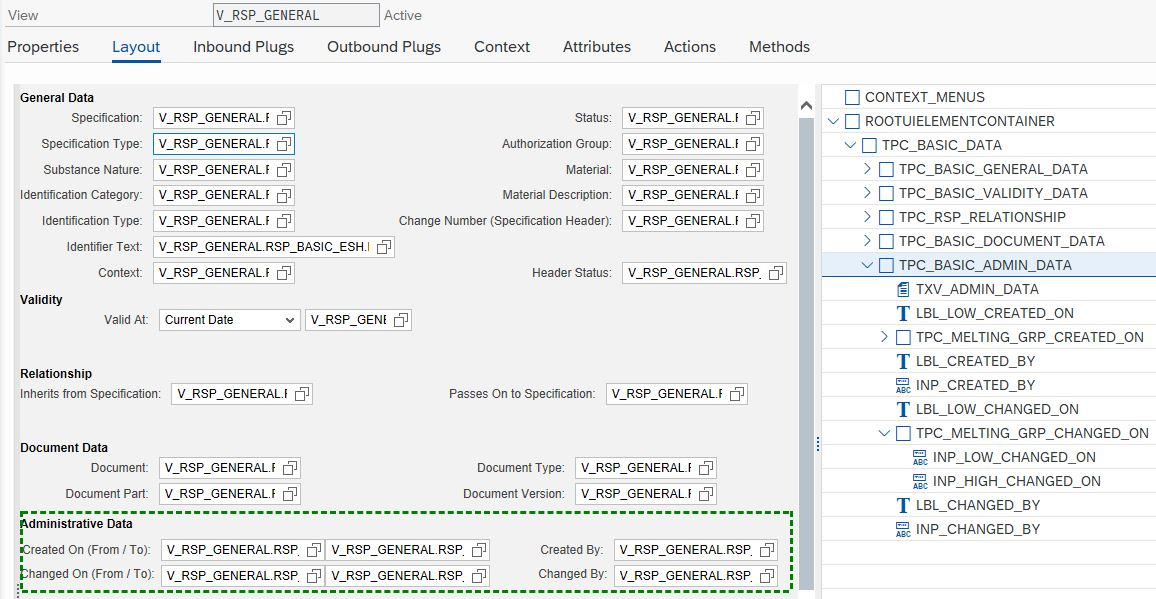
\includegraphics[width=1\textwidth]{img/NViewLayout.JPG}
    \caption[Aufbau der Suchoberfläche des General Views]{Aufbau der Suchoberfläche des General Views (Eigene Darstellung)}
    \label{fig:NViewLayout}
\end{figure}


Nach dem Erweitern des Range Views wurden die Suchkriterien changed on und changed by auch beim General View hinzugefügt. Hierzu wurde der in der Abbildung \ref{fig:NViewLayout} grün markierte Transportcontainer der Verwaltungsdaten \\TCP\_BASIC\_ADMIN\_DATA , um weitere \ac{ui}-Entitäten erweitert. Dabei war es besonders wichtig, 
die \ac{ui}-Entitäten INP\_LOW\_CHANGED\_ON und \\INP\_HIGH\_CHANGED\_ON in einem zusätzlichen Transportcontainer zu bündeln, damit die Eingabefelder wie gewünscht positioniert werden. Für den in der Abbildung \ref{fig:NViewLayout} rechts zu sehenden Aufbau des Layouts wurde auf die Erkenntnisse der Referenzmodellierung zurückgegriffen.


Um das Design der Suchoberflächen der Referenzmodelle beizubehalten, wurde insbesondere die Suchoberfläche der Materialstückliste eingehend untersucht. Hier standen vor allem die Attribute und Attributwerte der neuen Web-Dynpro-Entitäten im Vordergrund. Damit sich das \ac{ui} später dynamisch an die Größe des Screens anpassen kann und die zusammengehörenden Felder in einer Zeile dargestellt werden, wurde allen \ac{ui}-Entitäten eine prozentuale Breite zugewiesen. Darüber hinaus konnten bei der Betitelung der Labels erneut die bereits bekannten \acs{otr}-Texte wiederverwendet werden.

\begin{figure}[htbp]
    \centering
    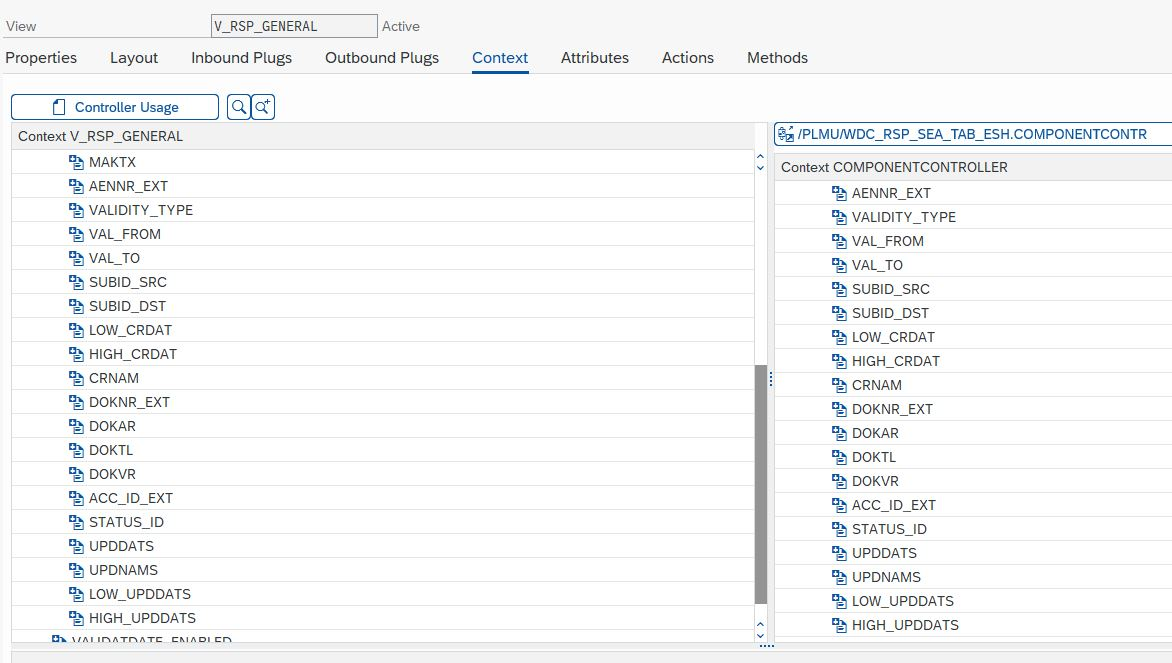
\includegraphics[width=1\textwidth]{img/ContextMapping.JPG}
    \caption[Context-Mapping zwischen dem View - und dem Component-Controller-Context]{Context-Mapping zwischen dem View - und dem Component-Controller-Context (Eigene Darstellung)}
    \label{fig:ContM}
\end{figure}

Nach der Konfiguration des Layouts war entscheidend, die Beziehungen der Web-Dynpro-Entitäten festzulegen, um das Transportieren der Eingabedaten innerhalb der Web-Dynpro-Component zu ermöglichen. Hierfür wurde zunächst das Mapping des Knotens RSP\_BASIC\_ESH im Component-Controller auf die \ac{ui}-Struktur aktualisiert, damit die neu angelegten Komponenten UPDDATS, LOW\_UPDDATS,  HIGH\_UPDDTAS und UPDNAMS für den General View zugänglich sind. Da die Context-Attribute des Component-Controllers nicht mehr mit den Context-Attributen des View-Controllers übereinstimmten, wurde das in Abbildung \ref{fig:ContM} zusehende Context-Mapping zwischen dem View-Context und dem Component-Controller-Context neu angelegt. Dadurch war es nachfolgend möglich, die Eingabefelder des Layouts mit den dazugehörigen Context-Attributen über ein Data-Binding zu verknüpfen.

Zudem waren noch analog zu den Referenzmodellen Anpassungen im Customizing für das Web \ac{ui} der Spezifikation erforderlich. Hier wurde für die Spezifikation der neue Suchbereich: RSP\_SELOPT angelegt. Für den Suchbereich wurde die Abfrageklasse /PLMI/CL\_RSP\_SEA\_CRIT\_SELOPT und \\/PLMB/CL\_SEA\_SELOPT\_CRIT\_DATA als Datenklasse mitgegeben, damit die zum Ausführen und Suchen von Daten benötigten Methoden der Suchanwendung mitgeteilt werden. Beide Klassen enthalten generische, sowie zusätzlich auf die Spezifikation zugeschnittene Methoden.

Um beide Views auf die neue Funktionalität testen zu können, wurde im Customizing über die Konfigurations-ID die zu den Views gehörenden Windows ausgewählt. Die Konfigurations-ID legt fest, welches Window beim Aufrufen der Suche im Browser angezeigt werden soll.

%Beim Testen wurden im \ac{plmwui} für die neuen Suchkriterien mehrere Werte und Wertebereiche ausgewählt und eine Suche angestoßen. Darauffolgend wurde die Liste der Ergebnisse durch Angeben zusätzlicher Sucheigenschaften weiter eingeschränkt, um das Zusammenspiel der neuen Suchkriterien mit den bereits vorhandenen überprüfen.


Zum Testen der neuen Suchfelder wurden im \ac{plmwui} zunächst einzelne Werte eingegeben und anschließend die Kriterien in Kombination mit anderen Suchkriterien getestet. Die im Webbrowser angezeigte Ergebnisliste wurde daraufhin mit den in der Datenbank vorliegenden Daten verglichen, um herauszufinden, ob die Suchanwendung vollumfänglich funktioniert.
%&Wenn die Ergebnisliste mit den Daten der Datenbank deckungsgleich ist, konnte Dadurch konnte auch bei einer Suche ohne Ergebnisse herausgefunden werden, ob für die Kombination von Suchkriterien tatsächlich kein Eintrag in der Datenbank vorliegt oder die Suchanwendung noch nicht funktioniert.

\begin{comment}
Beim Testen der Felder auf der Suchoberfläche der normalen View hat sich herausgestellt, dass für das Suchkriterium changed on keine Ergebnisse gefunden wurden, obwohl für den Zeitraum Einträge in der Datenbank vorlagen. Demzufolge wurde im \acs{abap} Editor mit dem Debuggen des Quellcodes begonnen und der erste Breakpoint in der Methode CL\_ESH\_TREX\_SEARCH gesetzt, um den Inhalt der Query zu überprüfen. (Die Query ist als Teil der ES zwischen der Suchanwendung und der Datenbank). Als Query wird die Tabelle bezeichnet, die die vom Benutzer für die Suchkriterien eingegebenen Werte, beinhaltet und das Übersetzen der Suchanfrage in ein SQL-Statement möglich macht.

Foto der Query einblenden

Nach dem eine weitere Suchanfrage gestartet wurde, konnte festgestellt werden, dass die Eingabedaten für das Feld changed on, die Query gar nicht erreichen und deshalb bei Suchanfragen nur leere Ergebnisse zurückgegeben werden. Daraufhin wurden die Methoden Schritt für Schritt durchlaufen und es hat sich herausgestellt, dass für die zwei Inputfelder des Suchkriteriums changed on zwei weitere Komponenten in der \ac{ui}-Struktur benötigt werden. Des Weiteren mussten die Komponentennamen mit LOW und HIGH beginnen, weil die Methode, die die Eingaben verarbeitet, ansonsten die beiden Datumseingaben nicht zu einem Zeitraum verknüpfen konnte.

Folglich wurde die\ac{ui}-Struktur um die Komponenten LOW\_UPDDATS und HIGH\_UPDDATS erweitert. Dabei wurde den Komponenten der Datentyp ESEUPDDAT zugewiesen, der zuvor auch für UPDDATS verwendet wurde. Anschließend mussten die Strukturänderungen durch das Aktualisieren der Mappings von Struktur zum ComponentControllerContext, von ComponentControllerContext zum ViewControllerContext und durch das Austauschen der Binding der Eingabefelder zum ViewControllerContext im WebDynpo Component verteilt werden.

% Code debuggt mit Variablen inhalten anzeigen und zusammenhänge der Methoden nach vollziehen, haben gezeigt, dass die Eingaben in der normalen View für changed on nur verarbeitet werden können wenn die vom \ac{ui} gebindetet Komponenten, die über den Componentcontroller auf die \ac{ui}-Struktur zeigen, mit LOW und HIGH beginnnen müssen. 
\end{comment}



Nachdem im Testverfahren, die Suche mit den hinzugefügten Kriterien einwandfrei funktionierte, wurden die Oberflächenanpassungen mithilfe der Transaktion SCWB in alle anderen Entwicklungssysteme der verschiedenen Releasestände transportiert. Da das Verteilen der Suchmodelländerungen nicht möglich ist, mussten in allen \ac{erp} und \acs{s/4hana} Entwicklungssystemen die Modellknoten manuell erweitert werden.


%In jedem Entwicklungssystem wird für jede Änderung am Suchmodell zur Laufzeit ein Report generiert;  Report könnte in andere Systeme transportiert werden
%Da die verschiedenen Entwicklungssysteme bei den gleichen Suchoberflächen unterschiedliche Suchkriterien haben können, lassen sich die Suchmodelländerungen nicht verteilen und mussten daher in allen \ac{erp} und \acs{s/4hana} Entwicklungsystemen manuell umgesetzt werden.


%früher hat man zu den Suchmodellen alle mglichen Felder hinzugefügt, und dann wurde darauf ein Index erzeugt
%Indixierungsprozess hat nachgeschaut, welche Felder brauchst du, sollen suchbar sein, 
%Früher müsste die Indixierungsprozess selbst geschrieben werden
% ERP Systeme: Suchmodelle von Anfang an mit vollumfänglicher Funktionalität und dafür auf maximale Effizienz im Indizierungsprozess verzichtet

%Nachdem die Übertragung der Änderungen in die verschiedenen Systeme abgeschlossen war, war es wichtig die fehlerfreie Funktionalität der neuen Felder in den Entwicklungssystemen zu kontrollieren. Die neuen Suchkriterien wurden mit mehreren Werten und Wertebereichen versehen und eine Suche angestoßen. Ebenfalls wurde die Liste der Ergebnisse durch Angeben zusätzlicher Sucheigenschaften weiter eingeschränkt um das Zusammenspiel der neuen Suchkriterien mit den bereits vorhandenen zutesten und zu überprüfen, ob die richtigen Ergebnisse dargestellt werden. Dabei hat sich herausgestellt, dass die automatische Zuweisung der Selektionshilfe bei dem Suchkriterium Changed by in der Normalen View nicht funktioniert. Infolgedessen wurde der Komponente UPDNAMS in der \ac{ui}-Struktur die ValueHelp manuell zugewiesen. Dabei konnte der Indentifikationsname der Changed on Valuehelp der Materialstückliste wiederverwendet werden. 

\begin{figure}[htbp]
    \centering
    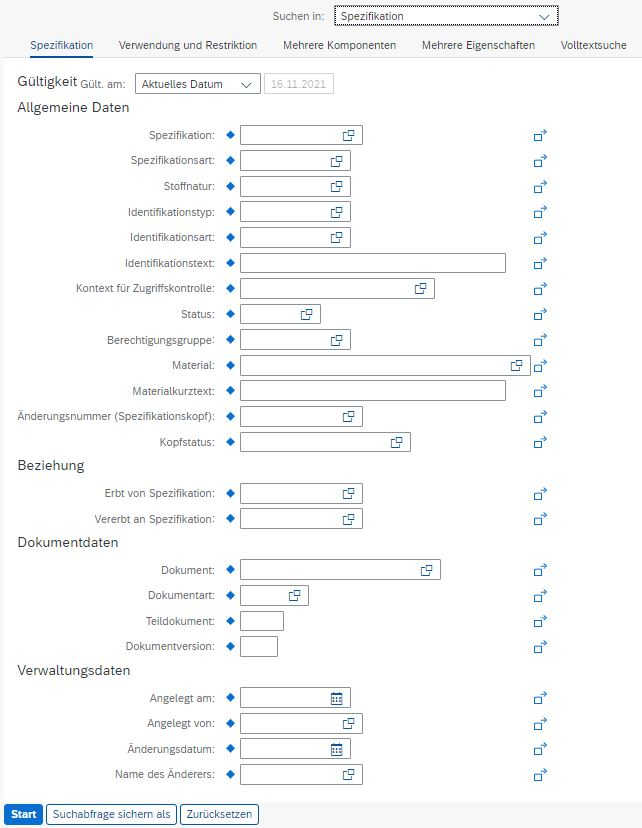
\includegraphics[width=0.9\textwidth]{img/LayoutRdanach2.jpg}
    \caption[Neue Suchoberfläche der PLM-Spezifikation im Range View]{Neue Suchoberfläche der PLM-Spezifikation im Range View (Eigene Darstellung)}
    \label{fig:Layoutfertig}
\end{figure}

Nach dem Übertragen der Anpassungen in die anderen Entwicklungssysteme war es noch einmal wichtig, das Coding und die Web-Dynpro Entitäten auch hier kurz zu überprüfen, um so die Vollständigkeit und Funktionalität der Suchoberflächen gewährleisten zu können. Anschließend war die Implementierung in den SAP-Entwicklungssystemen abgeschlossen. Das Ergebnis ist exemplarisch für den Range View in Abbildung \ref{fig:Layoutfertig} dargestellt.

Bevor die Übergabe an die Kunden erfolgen konnte, wurden die zur Auslieferung wichtigen Dokumente fertiggestellt und der Hinweis mit allen notwendigen Angaben befüllt. Dazu zählen die Information, die der Kunde zur Implementation und zum Nachvollziehen der Änderungen benötigt, sowie die Voraussetzungen, die Kundensysteme mitbringen müssen, um den Hinweis nutzen zu können.

Abschließend wurde mit dem Versenden des Hinweises und der Test Case Description die aktuell noch laufende Pilotrelease Phase angestoßen. 



%und die neue Funktionalität konnte aus den Entwicklungssystemen in die Qualitätssicherungssysteme übertragen werden.\change{auf Grafik eingehen} Dort wurden die gemachten Änderungen auf ihre Kompatiblilität mit anderen Systemen, die nicht direkt an der \ac{plmwui}-Suche beteiligt sind, überprüft, bevor die neue Funktionalität mit einem Hinweis in die Produktivsysteme der Kunden eingespielt werden konnte.

%Der Hinweis beinhaltet alle Informationen, die der Kunde benötigt, um die Änderungen bei sich erfolgreich einzuspielen. Dazu gehören Änderungen die der Kunde automatisch einspielen lassen kann, Informationen welche Hinweise der Kunde bereits benutzen muss und Anweisungen, die der Kunde nach implementieren des Hinweises noch manuell ausführen muss, um die Implementation abzuschließen. Somit hat der Kunde am Ende eine exakte Anleitung von SAP bekommen, mit der er die Lösung (zum Customer Connection Request) ohne Schwierigkeiten in seine Systeme implementieren kann.

\begin{comment}
Noch stärker differenzieren wo hat die Value Help funktioniert und wo nicht
Einleitung: Was muss umgesetzt werden 
Mögliche Themen zum ergänzen: Mandanten
Unklar wie aber Konnektoren größer aufziehen: Softwarekomponente wichtig, Status des Konnektors Möglichkeit zur Kontrolle ob dass indizieren und updaten funktioniert hat
Neben Binding Mapping erklären
Reihenfogle entscheidend
F4 Hilfe manuell hinzugefügt, da dass mit dem System nicht funktioniert hat
Testen der Funktionalität mit hilfe der ESTRH Tabelle, Datenbank im ABAPEditor anschauen:
    Hier gemachte Suchanfragen mit denen im Web \ac{ui} vergleicht und dann verglichen ob die Ergebnisse die gleichen sind, beziehungsweise ob die Spezifikationen, die mir nicht angezeigt werden, aufgrund vonmangelder Berechtigung verborgen werden oder eben die Suche noch nicht zu 100 \% funktioniert
    Welche Kombinationen ausprobiert, worauf geachtet und Sterne erklären: 
        Beachten Sie, dass sich die Suche in Dokumenten und die Suche in Textfeldern von Business-Objekten leicht unterscheiden. Textfelder werden in der Regel als Strings indiziert und Suchbegriffe müssen mit diesen Strings komplett übereinstimmen. Texte dagegen werden in einzelne Wörter aufgespalten, bevor sie indiziert werden, und selbst Wortkombinationen werden aufgespalten. Wenn Sie sicherstellen möchten, dass bei einer Suche in Business-Objekten alle Kombinationen Ihres Begriffs gefunden werden, müssen Sie ihn in Sterne setzen, z.B. *abc*. Das ist bei einer Suche in Dokumenten nicht notwendig.

Teil der Systeme als Pilotrelease an den Kunden rausgeschickt, feedback bekommen das die Note funktionier
testen imProduktivsystem

Umgehen und setzten von breakpoints

\end{comment}